%-------------------------------------------------------------
% CV en español
% Hugo Ferrando Seage - 2016
%-------------------------------------------------------------

\documentclass[a4paper, 11pt]{article}
\usepackage[utf8]{inputenc}
\usepackage[T1]{fontenc}
\usepackage[spanish]{babel}
\usepackage{subfig}
\usepackage{booktabs}
\usepackage{enumitem} % Customize enumerate items
\usepackage{longtable} % Required to make tables span more than one page
\usepackage{graphicx} % Required for including pictures
\usepackage[cm]{fullpage}
\usepackage[usenames,dvipsnames]{xcolor} % Required for specifying custom colors
\usepackage[pdfstartview=Fit]{hyperref} % Required for adding links	and customizing them
\definecolor{linkcolour}{rgb}{0,0.2,0.6} % Link color
\hypersetup{colorlinks,breaklinks,urlcolor=linkcolour,linkcolor=linkcolour, pdfpagemode=UseNone} % Set link colors throughout the document
\hyphenpenalty=10000

\begin{document}
\pagestyle{empty} % Removes page numbering

\begin{flushright}
    Estudiante de 4\textsuperscript{o} curso\\
    Grado en Ingeniería Informática\\
    +34 680 340 463\\
    \href{mailto: me@hugofs.com}{me@hugofs.com}\\
    \href{mailto: hugoseage@gmail.com}{hugoseage@gmail.com}\\
    \href{https://hugofs.com}{hugofs.com}\\
\end{flushright}

\vspace{-40mm}

\begin{figure}[ht!]
    \begin{flushleft}
        \subfloat{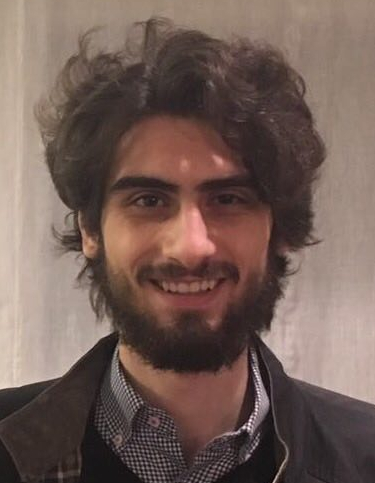
\includegraphics[width=0.13\textwidth]{images/hugo.jpg}}
    \end{flushleft}
\end{figure}

{\textsc {\Huge \vspace{5mm} \hspace{-13mm} Hugo Ferrando Seage}}\\

\begin{longtable}{rp{11cm}}
    EXPERIENCIA
    & {\bf Beca de investigación en la UEM} \hfill sep 16 --- mar 17\\
    & Modelo de predicción de gustos de usuarios a partir de textos de opinión en Amazon, usando sistemas distribuidos\\
    \\
    & {\bf Telefónica --- Talentum Startups} \hfill sep 16 --- mar 17\\
    & Mejoras del sistema de recomendación content-to-content de \href{http://ver.movistarplus.es/}{Movistar+}\\
    \\
    & {\bf Beca de investigación en la UEM} \hfill ago 16 --- sep 16\\
    & Detección de personas en piscinas y playas usando OpenCV para dron salvavidas\\
    \\
    & {\bf Desarrollador web en Product Hackers} \hfill jun 16 --- oct 16\\
    & Creación de web apps y chat bots usando Angular 2 y Ionic 2 para móviles y web\\
    \\
    & {\bf Beca de investigación en la UEM} \hfill sep 15 --- ene 16\\
    & Desarrollo de una app para detectar, alertar y registrar infracciones de tráfico usando OpenCV en Android (visión e inteligencia artificial)\\
    \\
    EDUCACIÓN
    & {\bf Universidad Europea de Madrid} \hfill 2014 --- 2017\\
    & Grado en Ingeniería Informática\\
    \\
    & {\bf Universidad Politécnica de Madrid} \hfill 2012 --- 2014\\
    & Grado en Ingeniería Informática\\
    \\
    CONOCIMIENTOS TÉCNICOS
    & {\bf Lenguajes de Programación}\\
    & Python, C/C++, Java, Bash, Javascript/NodeJS, Typescript\\
    \\
    & {\bf Frameworks}\\
    & Apache Spark, Angular 2, Ionic 2, Spring, NLTK, Bootstrap, jQuery\\
    \\
    & {\bf Herramientas}\\
    & Git, SSH, GPG, \LaTeX, Android SDK \& NDK, Nginx, Jenkins, OpenVPN, Knot, Unbound, Btrfs\\
    \\
    & {\bf Sistemas Operativos}\\
    & GNU/Linux, Microsoft Windows, Android\\
    \\
    PROYECTOS
    & \vspace{-8mm}
    \begin{itemize}[leftmargin=0cm,label={}]
        \item \href{https://github.com/hugo19941994/CHIP8-Emu}{Intérprete CHIP-8}: Ejecuta programas de CHIP-8 en Windows y Linux
        \item \href{https://github.com/hugo19941994/SpaceInvaders-Emu}{Emulador Intel 8080}: Ejecuta Space Invaders en Windows
        \item ovpn.io: Proveedor de VPN basadas en OpenVPN (offline)
        \item \href{https://github.com/hugo19941994/ViajeFacil}{ViajeFácil}: Software de gestión para agencias de vuelos. Colaboración entre UEM \& Unisys
        \item \href{https://github.com/hugo19941994/CV-Parser}{CV-Parser}: Sistema para gestionar CV usando reconocimiento de entidades nombradas y redes bayesianas. Colaboración entre UEM \& Everis
        \item \href{https://github.com/hugo19941994/robot}{Human Rescue Bot}: Ganador del Laureate Awards for Excellence in Robotics Engineering 2016
    \end{itemize}\\
    \\
    CERTIFICACIONES
    & \vspace{-8mm}
    \begin{itemize}[leftmargin=0cm,label={},noitemsep]
        \item Certificate in Advanced English (CAE)
        \item CCNA 1: Introduction to Networks
        \item CCNA 2: Routing and Switching Essentials
        \item CCNA 4: Connecting Networks
    \end{itemize}\\
    \\
    IDIOMAS
    & \vspace{-8mm}
    \begin{itemize}[leftmargin=0cm,label={},noitemsep]
        \item Español nativo
        \item Inglés avanzado
        \item Italiano nativo
        \item Francés básico
    \end{itemize}
\end{longtable}
\end{document}
